\documentclass[10pt]{article}
\usepackage[utf8]{inputenc}
\usepackage[activeacute,spanish]{babel}
\usepackage[left=1.5cm,top=1.5cm,right=1.5cm, bottom=1.5cm,letterpaper, includeheadfoot]{geometry}

\usepackage{amssymb, amsmath, amsthm}
\usepackage{graphicx}
\usepackage{hyperref}
\usepackage{lmodern,url}
\usepackage{paralist} %util para listas compactas
\usepackage{xcolor}
\usepackage{bbm}
\usepackage{mathrsfs}
\usepackage{bbm}

%========PAQUETES AGREGADOS===========
%Pseudocodigo
\usepackage{pseudocode}
\usepackage[portuguese, boxruled]{algorithm2e}
\usepackage{wrapfig}
\usepackage{multicol}
\usepackage{graphicx}
\usepackage{caption}
\usepackage{subcaption}
%\captionsetup[table]{labelformat=empty}
\captionsetup[subfigure]{labelformat=empty}
\usepackage{cancel}
\usepackage{tikz}
\def\checkmark{\tikz\fill[scale=0.4](0,.35) -- (.25,0) -- (1,.7) -- (.25,.15) -- cycle;} 
%====================================

\usepackage{fancyhdr}
\pagestyle{fancy}
\fancypagestyle{plain}{%
\fancyhf{}
\lhead{\footnotesize\itshape\bfseries\rightmark}
\rhead{\footnotesize\itshape\bfseries\leftmark}
}


% macros
\newcommand{\Q}{\mathbb Q}
\newcommand{\R}{\mathbb R}
\newcommand{\N}{\mathbb N}
\newcommand{\Z}{\mathbb Z}
\newcommand{\C}{\mathbb C}
\newcommand{\BigO}{\mathcal{O}}
%Teoremas, Lemas, etc.
\theoremstyle{plain}
\newtheorem{teo}{Teorema}
\newtheorem{lem}{Lema}
\newtheorem{prop}{Proposición}
\newtheorem{cor}{Corolario}
\newtheorem{obs}{Observación}
\newtheorem{ej}{Ejemplo}
\renewcommand{\qedsymbol}{\rule{0.7em}{0.7em}}
\renewenvironment{proof}{{\bfseries \noindent Demostración}}{ \qed \\}


\theoremstyle{definition}
\newtheorem{defi}{Definición}
% fin macros


\newcommand{\catnum}{8} %numero de catedra
\newcommand{\fecha}{13 de Septiembre 2016 }

%%%%%%%%%%%%%%%%%%

%Macros para este documento
\newcommand{\cin}{\operatorname{cint}}



\begin{document}
%Encabezado
\fancyhead[L]{Facultad de Ciencias Físicas y Matemáticas}
\fancyhead[R]{Universidad de Chile}
\vspace*{-1.2 cm}
\begin{minipage}{0.6\textwidth}
\begin{flushleft}
\hspace*{-0.5cm}\textbf{MA3402-1 Estadística. Primavera 2016}\\
\hspace*{-0.5cm}\textbf{Profesor:} Raul Gouet\\
\hspace*{-0.5cm}\textbf{Escriba:} Manuel Cáceres\\
\hspace*{-0.5cm}\textbf{Fecha:} \fecha
\end{flushleft}
\end{minipage}
\begin{minipage}{0.36\textwidth}
\begin{flushright}

\includegraphics[scale=0.3]{imagenes/fcfm_dcc}
\end{flushright}
\end{minipage}
\bigskip
%Fin encabezado

\begin{center}
\LARGE\textbf{Clase \catnum}
\end{center}
\section{Continuamos con intervalos de confianza}
$X_{1},X_{2},\ldots,X_{n}$ iid $N(\mu,\sigma^2)$, $\theta = (\mu,\sigma) \in \mathbb{R}\times(0,\infty)$, ambos desconocidos. Queremos un intervalo para $\mu$ y en el caso de $\sigma$ conocido, usamos el pivote:
\begin{align*}
T(x,\mu) = \sqrt{n} \frac{\bar{X}-\mu}{\sigma}
\end{align*}
Podemos, si $\sigma$ desconocido, reemplazar $\sigma$ por $\hat{\sigma}$ (algún estimador).\\
Usar como pivote la función
\begin{align*}
\tilde{T} = \sqrt{n} \frac{\bar{X}-\mu}{\hat{\sigma}}
\end{align*}
Hay que asegurar que $\tilde{T}$ tenga:
\begin{enumerate}
\item Distribución independiente de $\theta$
\item Sea monótona en $\mu$
\end{enumerate}
No sabemos si se puede resolver/determinar $t_{\alpha_{1}}, t_{\alpha_{2}}$ tales que $\mathbb{P}_{\theta}(t_{\alpha_{1}}\le \tilde{T}(x,\mu\le t_{\alpha_{2}})\ge 1-\alpha$
\begin{center}
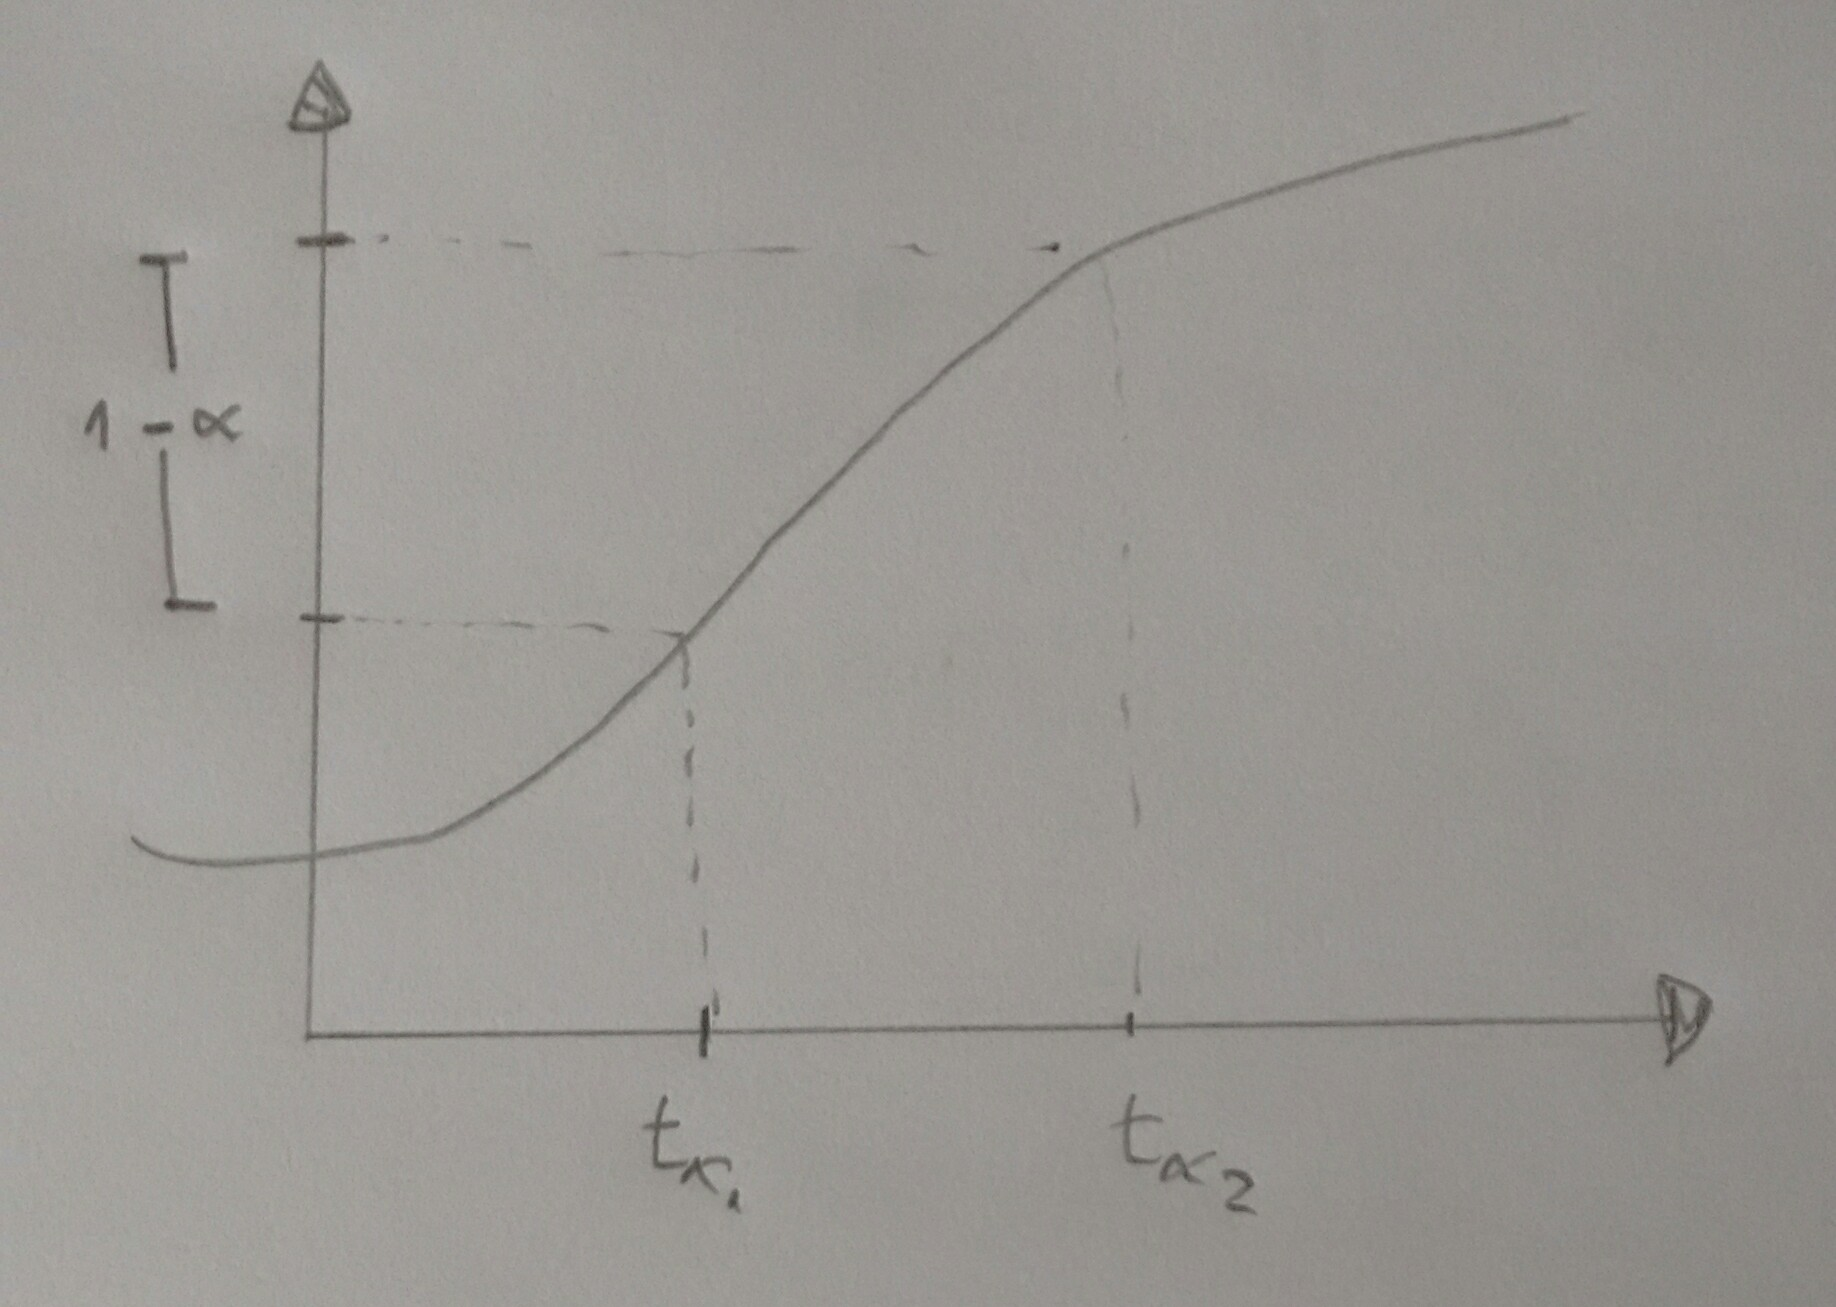
\includegraphics[scale=0.2]{imagenes/distr1.jpg}
\end{center}
Para obtener las condiciones anteriores se usa el estimador $\sigma^2$.
\begin{align*}
\hat{\sigma}^2 = \frac{1}{n-1}\sum_{i=1}^n {(X_{i}-\bar{X})^2}
\end{align*}
Sabemos $\hat{\sigma}^2$ es insesgado para $\sigma^2$ y de hecho es el EIVUM, etc. No sabemos como incide esto en los intervalos.\\

Se puede demostrar el siguiente resultado (postergaremos la demostración para el capítulo de modelos lineales).\\

La variable aleatoria $\sum_{i=1}^n {\frac{(X_{i}-\bar{X})^2}{\sigma^2}}$ se distribuye como una $\chi^2(n-1)$ (chi cuadrado con $n-1$ grados de libertad). Pero una $chi^2$ es una $\Gamma (\lambda,p) \rightarrow \frac{\lambda(\lambda x)^{p-1}e^{-\lambda x}}{\Gamma (p)}, x \ge 0$.\\
Además demuestra que $\bar{X}$ y $\sum_{i=1}^n {(X_{i}-\bar{X})^2}$ son variables aleatorias independientes.\\

Se introduce la variable llamada $t$ de student.\\
 Dadas $X \sim N(0,1), Y \sim \chi^2(n)$, se define la variable aleatoria $T$ con densidad $t$ e student con $n$ grados de libertad, como
 \begin{align*}
 T = \frac{X}{\sqrt{\frac{Y}{n}}}
 \end{align*}
 Volvamos al pivote $\tilde{T}$:
 \begin{align*}
 \tilde{T} = \frac{\bar{X}-\mu}{\frac{\hat{\sigma}}{\sqrt{n}}} = \sqrt{n}\frac{\left(\frac{\bar{X}-\mu}{\sigma}\right)\sim N(0,1)}{\sqrt{\frac{\sum_{i=1}^n {(X_{i}-\bar{X})^2}}{\sigma^2(n-1)}}\sim \sqrt{\frac{\chi^2(n-1)}{n-1}}}
 \end{align*}
 Lo anterior muestra que $\tilde{T}$ tiene una ley $t$ de student con $n-1$ grados de libertad. Escribimos $\tilde{T} \sim t(n-1)$.\\
 Designemos por $\Phi_{n}$ la función de distribución de una variable aleatoria $t(n)$.\\
 
 Ahora seguimos el cálculo buscando $t_{\alpha_{1}}, t_{\alpha_{2}}$ tales que:
 \begin{align*}
 \mathbb{P}_{\theta}(t_{\alpha_{1}} \le \tilde{T}(x,\mu) \le t_{\alpha_{2}}) = \Phi_{n-1}(t_{\alpha_{2}}) - \Phi_{n-1}(t_{\alpha_{1}}) = 1-\alpha
 \end{align*}
 Obtenemos el siguiente intervalo para $\mu$:
 \begin{align*}
 [\bar{X}- t_{\alpha_{2}}\frac{\hat{\sigma}}{\sqrt{n}}, \bar{X}- t_{\alpha_{1}}\frac{\hat{\sigma}}{\sqrt{n}}]
 \end{align*}
 Si optimizamos el largo llegamos a una solución casi idéntica al caso $\sigma$ conocido pero usando la $t$ de student en lugar de la normal, obteniendo :
  \begin{align*}
 [\bar{X}- t_{\alpha/2}\frac{\hat{\sigma}}{\sqrt{n}}, \bar{X}+ t_{\alpha/2}\frac{\hat{\sigma}}{\sqrt{n}}]
 \end{align*}
 \begin{center}
 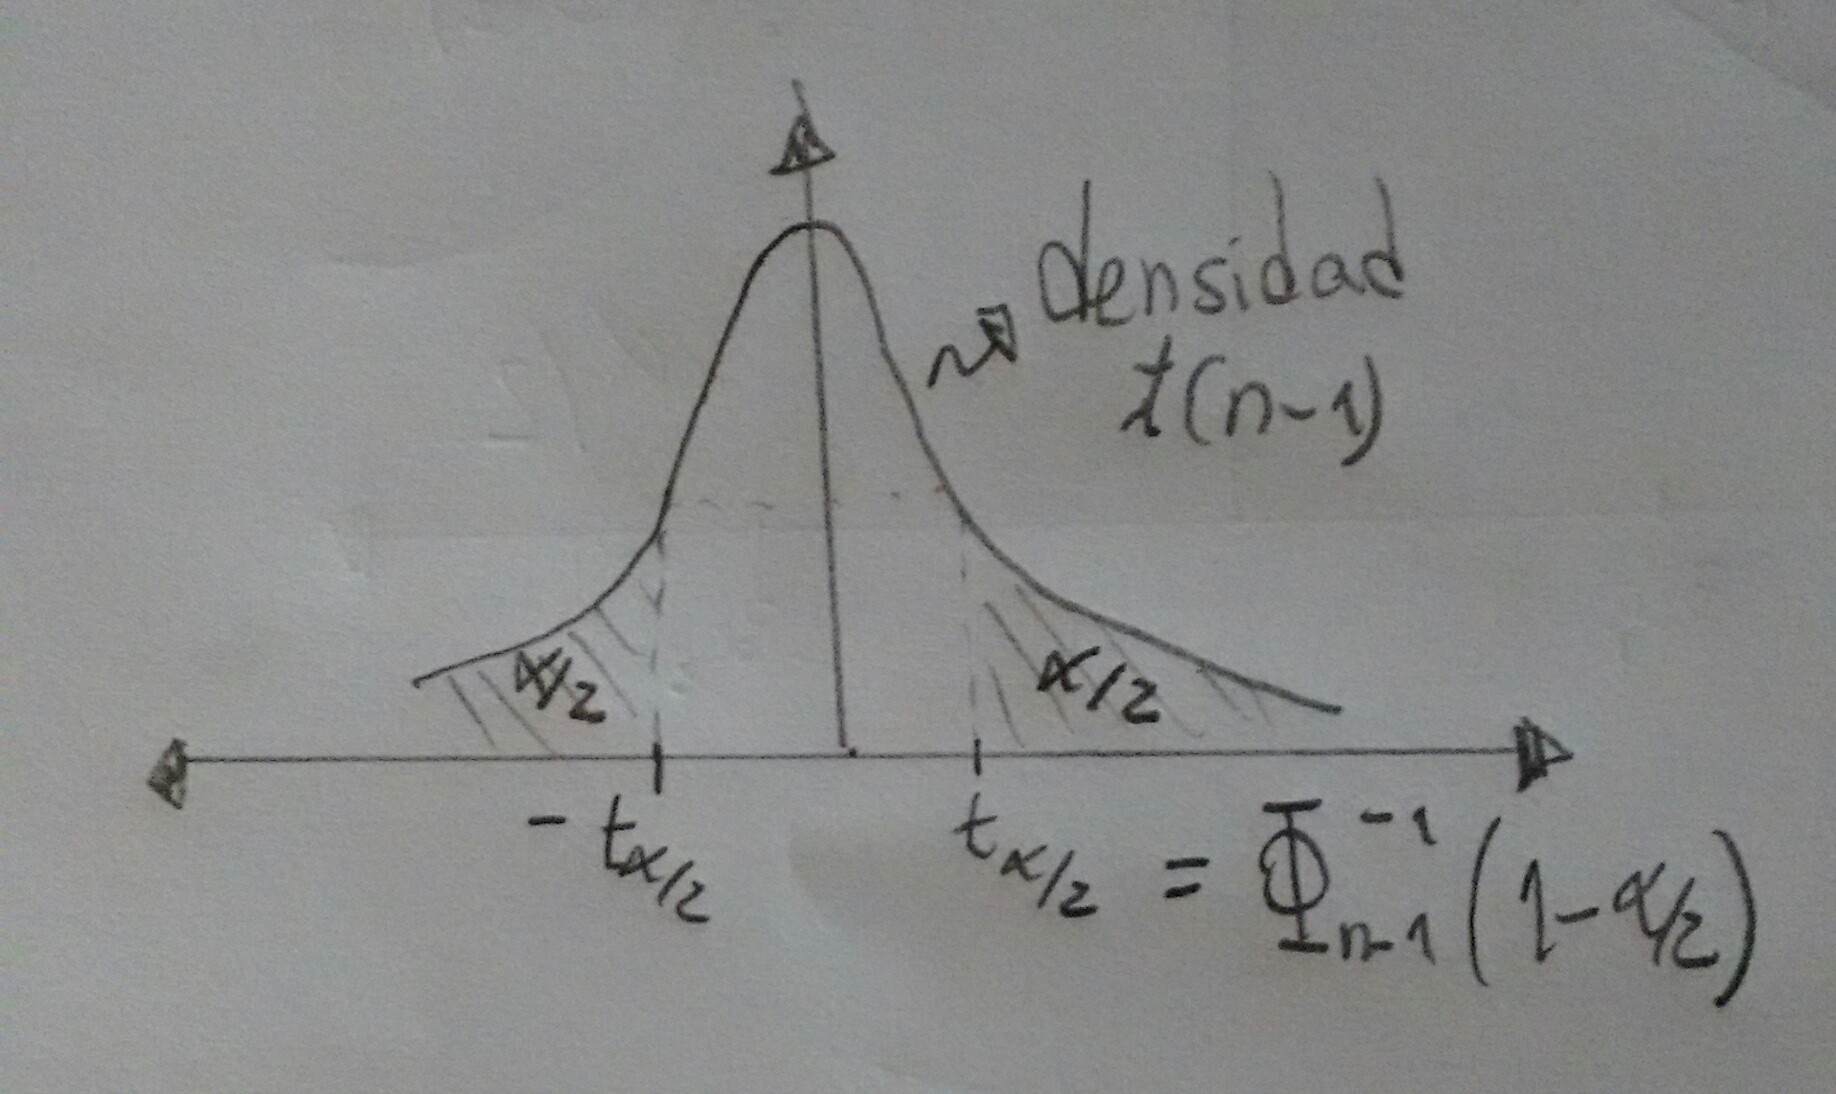
\includegraphics[scale=0.2]{imagenes/distr2.jpg}
 \end{center}
 Terminemos con un ejemplo de pivote para $\sigma^2$ en la normal $N(\mu,\sigma^2)$.\\
 Aprovechemos que $\sum {\frac{(X_{i}-\bar{X})^2}{\sigma^2}} \sim \chi^2(n-1)$.\\
 Definimos el pivote:
 \begin{align*}
 S(x,\sigma) = \frac{\sum {(X_{i}-\bar{X})^2}}{\sigma^2}
 \end{align*}
 \begin{itemize}
 \item Es función decreciente de $\sigma$
 \item Su distribución no depende de $\theta = (\mu,\sigma)$
 \end{itemize}
 Esto se puede usar para definir un intervalo para $\sigma^2$.\\
 Lo malo es que no hay simetría y resulta más dificil optimizar el largo:
 \begin{align*}
 \mathbb{P}_{\theta}(X_{\alpha_{1}}\le \sum {\frac{(X_{i}-\bar{X})^2}{\sigma}} \le X_{\alpha_{2}}) = 1-\alpha
 \end{align*}
 \begin{center}
 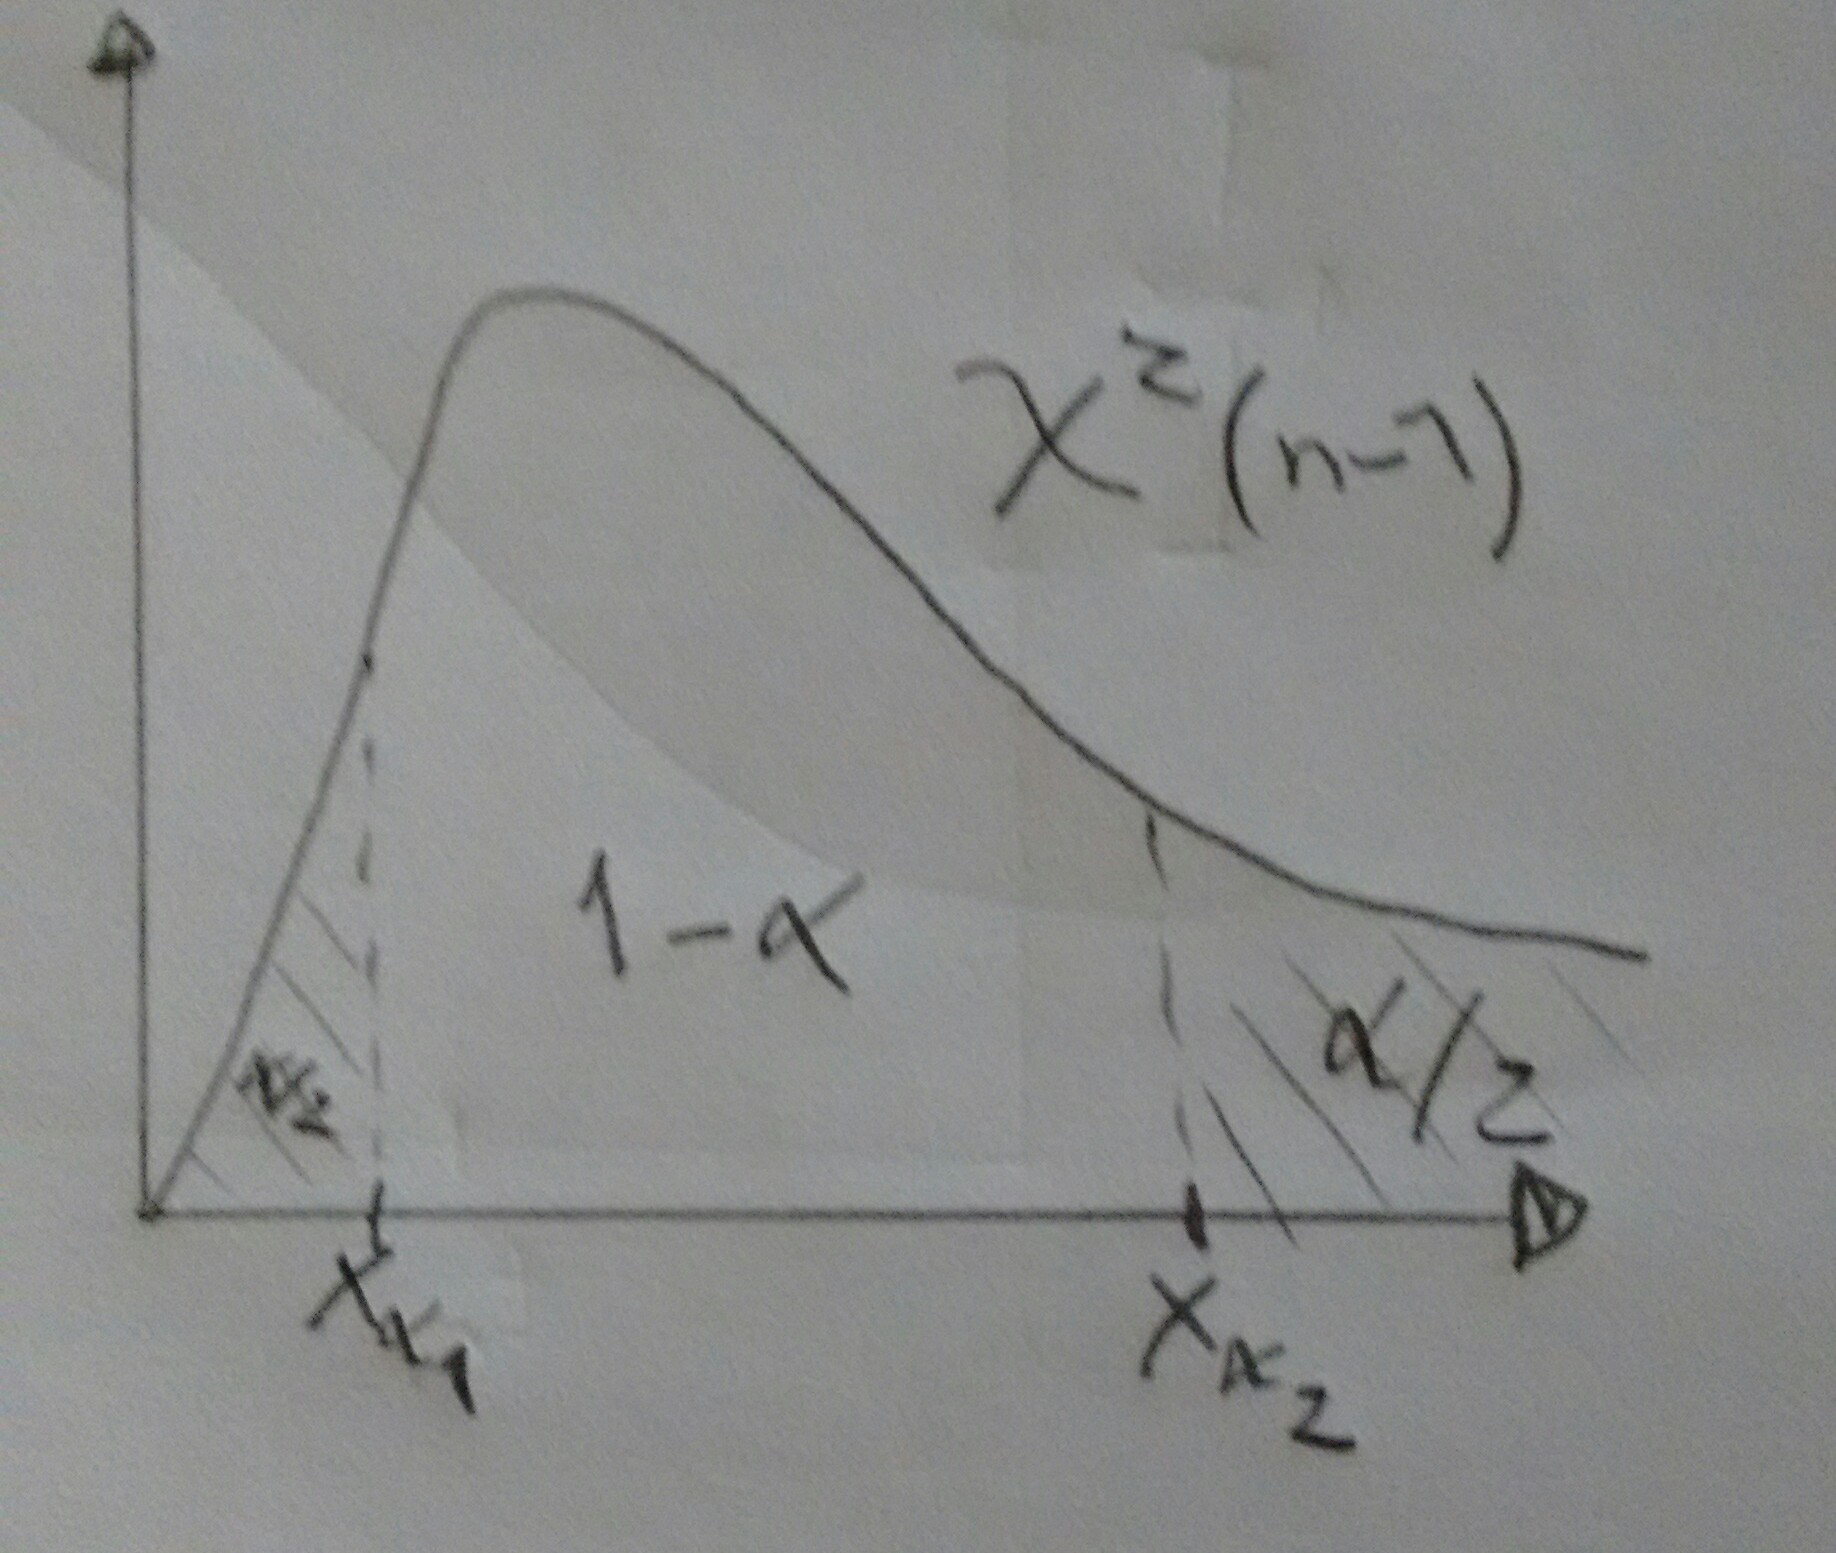
\includegraphics[scale=0.2]{imagenes/distr3.jpg}
 \end{center}
 \section{Test de Hipótesis}
 Veremos la teoría de Neyman-Pearson.\\
 
 Comenzamos con el modelo paramétrico $\mathcal{P} = \{\mathbb{P}_{\theta}\colon \theta \in \Theta\}$ y consideramos una partición en dos $\Theta_{0}$ y $\Theta_{1}$.\\
 
 El problema es ``Adivinar'' (estimar) en cual de los dos conjuntos está el verdadero $\theta$, ya no importa estimar $\theta$, sino que asignarlo a uno de estos conjuntos.\\
 
 Tenemos la observación $X$ y queremos decidir, usando $X$ si postulamos $\theta \in \Theta_{0}$ o bien $\theta \in \Theta_{1}$.
 
 \begin{ej}
 Se lanza una moneda $n$ veces independientemente.\\
 Tenemos modelo clásico.
 \begin{align*}
 \mathbb{P}_{\theta}(X=x) = \theta^{\sum X_{i}}(1-\theta)^{n-\sum X_{i}},\ X_{i}\in \{0,1\}
 \end{align*}
 Sea $\Theta = [0,1], \Theta_{0} = [1/2-\epsilon, 1/2+\epsilon], \Theta_{1} = \Theta \setminus \Theta_{0}$.\\
 Se plantea la siguiente estrategia de decisión:\\
 Si $\bar{X}\in \Theta_{0}$ declaro $\theta \in \Theta_{0}$, si no $\theta \Theta_{1}$
 \end{ej}
 \section{Algunas definiciones}
 Se consideran dos hipótesis asociadas a la partición $\{\Theta_{0},\Theta_{1}\}$ de $\Theta$.\\
 La hipótesis ``nula'' se designa por $H_{0}$, corresponde a $\Theta_{0}$ y escribimos $H_{0}\colon \theta \in \Theta_{0}$.\\
 La hipótesis ``alternativa'' se designa por $H_{1}$, corresponde a $\Theta_{1}$ y escribimos $H_{1}\colon \theta \in \Theta_{1}$.\\
 
 Al plantear el problema de test de hipótesis se dice que tenemos $H_{0}\colon \theta \in \Theta_{0}$ versus $H_{1}\colon \theta \in \Theta_{1}$.\\
 
 Disponemos de la observación $X$ pero necesitamos una regla de desición (que llamaremos test) donde participe $X$.\\
 
 Un test es una función $\Phi: \mathfrak{X}\mapsto\{0,1\}$. Esta función se aplica como sigue:
 \begin{itemize}
 \item Si $\Phi(x)=0$ entonces no rechazamos $H_{0}$ (nos quedamos con $H_{0}$).
 \item Si $\Phi(x)=1$ entonces rechazamos $H_{0}$ (nos quedamos con $H_{1}$).
 \end{itemize}
 Tradicionalmente se define
 \begin{align*}
 \mathbb{R}_{\Phi}= \{x\in \mathfrak{X}\colon \Phi(x)=1\} = \Phi^{-1}(1)
 \end{align*}
 y se llama región crítica o de rechazo del test $\Phi$. $\mathbb{R}_{\Phi}$ es la colección de todas las observaciones que llevan a rechazar $H_{0}$.
 \subsection{Errores}
 Reconocemos dos tipos de errores en este contexto.
 \begin{enumerate}
 \item Diremos que se comete error tipo I, cuando se rechaza $H_{0}$, pero $H_{0}$ es cierto.
 \item Diremos que se comete error tipo II, cuando no se rechaza $H_{0}$, pero $H_{0}$ es falsa.
 \end{enumerate}
 \begin{center}
 \begin{tabular}{c|c|c}
 & $H_{0}$ & $H_{1}$ \\ \hline
 Rechazar $H_{0}$ & I & \checkmark \\ \hline
 No rechazar $H_{0}$ & \checkmark & II
 \end{tabular}
  \end{center}
 Lo que queremos es encontrar test $\Phi$ con baja probabilidad de error.\\
 Primero veamos la probabilidad de rechazar.\\
 Recordemos que se rechaza $H_{0}$ si $\Phi(x) = 1$ o si $x \in \mathbb{R}_{\theta}$.Entonces:
 \begin{align*}
 \alpha_{\Phi}(\theta) := \mathbb{P}_{x\in \mathbb{R}_{\theta}} = \mathbb{E}_{\theta}(\Phi(x))
 \end{align*}
 Si $\theta \in \Theta_{0}$, entonces $\alpha_{\Phi}(\theta)$ es la probabilidad de rechazar cuando no debemos, luego quisieramos que $\alpha_{\Phi}(\theta)\approx 0, \forall \theta \in \Theta_{0}$. Con esto controlamos el error tipo I.\\
 
 Por otra parte si $\theta \in \Theta_{1}$ quisieramos que $\alpha_{\Phi}(\theta)\approx 1$.\\
 
 Así, el test ideal $\Phi$ debería tener $\alpha(\theta)= 0 \forall \theta \in \Theta_{0}$ y $\alpha(\theta)=1 \forall \theta \in \Theta_{1}$.\\
 Se demuestra que no existe el test ideal (salvo casos artificiales) y buscamos alternativas:
 \begin{center}
 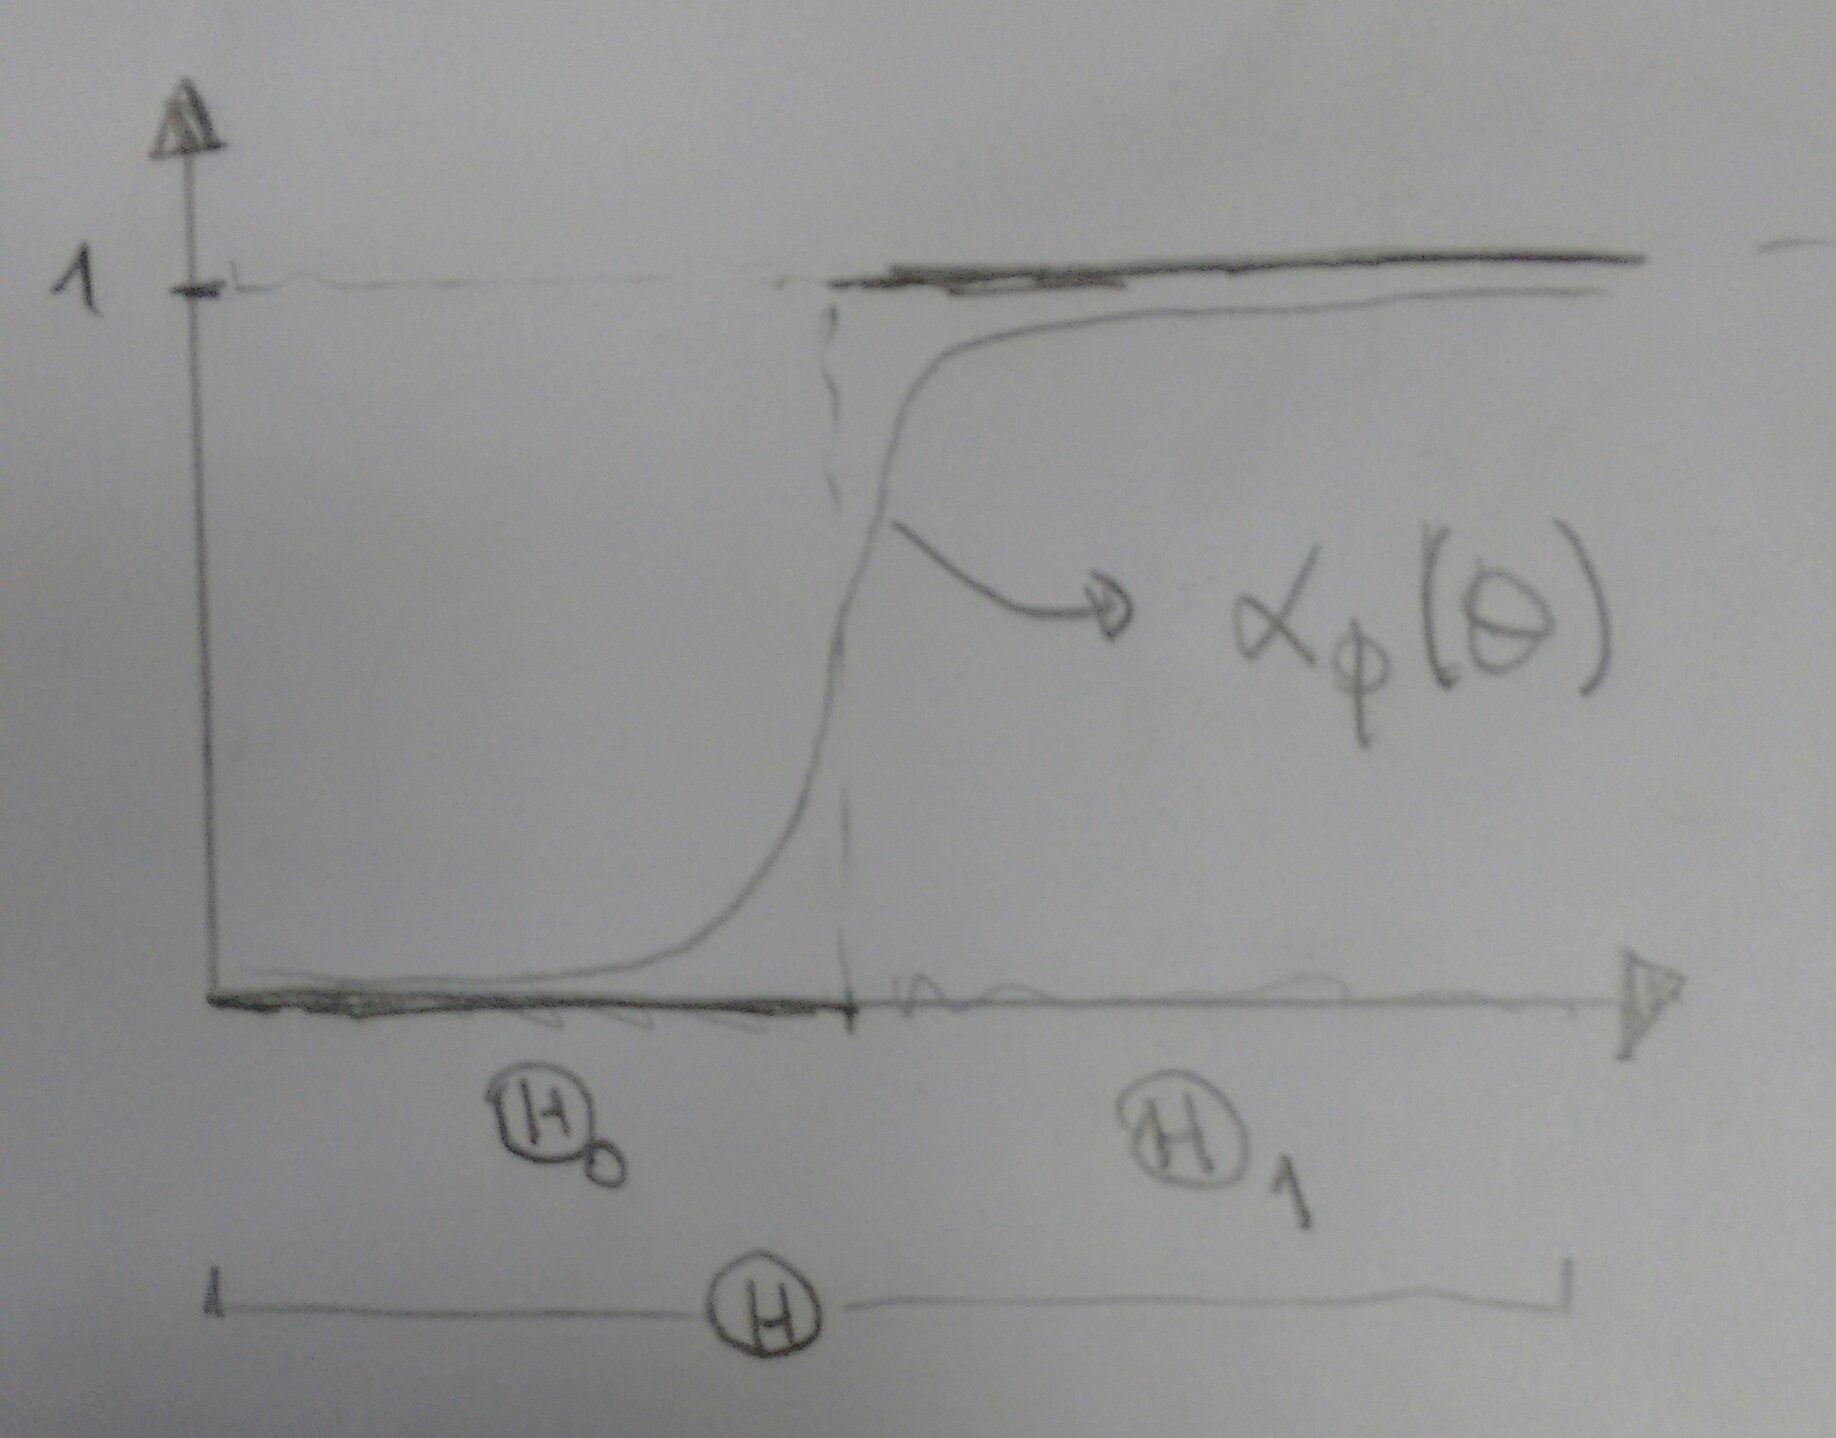
\includegraphics[scale=0.2]{imagenes/test1.jpg}
 \end{center}
\end{document}
